\documentclass{article}
%\usepackage{geometry}
%\geometry{top = 1in, bottom = 1in, left = 1in, right = 1in}
\usepackage[top = 0.7in, bottom = 0.7in, left = 0.7in, right = 0.7in]{geometry}
\usepackage{amsmath,amssymb,amsthm,mathrsfs}
\usepackage{graphicx}
\usepackage{bm}
\usepackage{float}
\usepackage[font=footnotesize,labelfont=bf]{caption}
\usepackage{movie15}
\usepackage{hyperref}

\usepackage{fancyhdr}
\pagestyle{fancy}
\rhead{\footnotesize {february 2018} }
\chead{\footnotesize {Authors: Anne Thoul} }
\lhead{\footnotesize {mesa/star/test\_suite/semiconvection} }

\begin{document}
	
	\begin{center}
	  \begin{Large}
	    \textbf{Semiconvection}\\
	  \end{Large}
	\end{center}


This test is to show the capability of MESA to correctly place the convective and semiconvective boundaries using the Ledoux criterion and predictive mixing (see MESAIV paper), and allow mixing from semiconvection according to the Langer prescription.\\

It evolves a 1.5M model from zero age main sequence to when the central hydrogen mass fraction drops below 0.4. At that time the convective core has almost (but not quite) reached its maximum mass extension, and there is a semiconvective layer above the convective core.\\

To verify that the test ran successfully, MESA checks the mixing types at three points (0.12, 0.135, and 0.15Msun), where the convective types should be convection, semiconvection, and no mixing, and the average temperature and density between two points in the star. Target values and ranges are listed in src/run\_star\_extras.f. If the mixing types match and the temperature and density values fall within the given range, the terminal output at the end of the run should read "all values are within tolerances".\\

The inlist used to produce the starting zams model (inlist\_to\_ZAMS) is provided.\\

Note that the choice made for the inital mixture (a09 in this test case) and for the nuclear reaction network (here: \texttt{pp\_and\_cno\_extras.net}) influence the growth of the convective core (see below). The values used in this test case for the \texttt{predictive\_superad\_thresh} parameters work well here but need to be adjusted when using other mixtures or nuclear reaction networks.\\

Note also that for speed purposes the values used here for the maximum allowed timestep and the mesh size do not produce completely converged models, in particular at the beginning of the evolution (as shown in cyan in fig.\ref{fig:2}). A convergence study should be done when using this inlist for science purposes.\\

 \pagebreak
 
{\bf Influence of initial mixture}:\\

Given the strong dependence of the radiative temperature gradient on the opacities, the results are quite different when using different mixtures. In figure \ref{fig:1} we show the results obtained using the gs98 and the a09 mixtures. 

The red and green lines show the convective (plain lines) and semiconvective (dotted lines) boundaries using the gs98 mixture for two different values of \texttt{predictive\_superad\_thresh} (0.001 and 0.005).
The blue lines show the result obtained using the a09 mixture.

Note that the size of the convective core depends in a significant way on the mixture used.
Note also that the \texttt{predictive\_superad\_thresh}  value that should be used to avoid the splittings (seen in the red case) depends on the mixture used. The value  0.001 works well for the a09 mixture, but a larger value is needed when using the gs98 mixture.

 \begin{figure}[H]
	    \centering
	    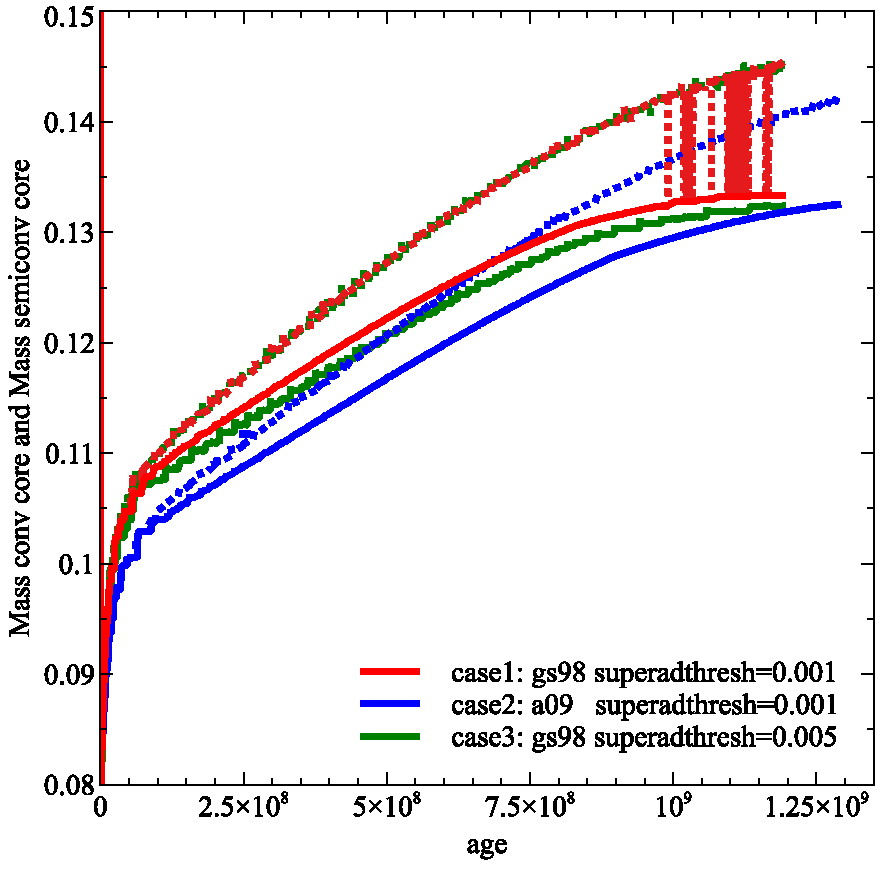
\includegraphics[width = 3.8in]{mixture.pdf}
	    \caption{}
	    \label{fig:1}
 \end{figure}


 \pagebreak
 
{\bf Influence of nuclear reaction network}:\\

The choice of nuclear reaction network also has a non negligible influence on the size of the convective core.
In fig.\ref{fig:2}, the a09 mixture was used, with two different nuclear reaction networks. 

In red the results obtained using the MESA default reaction net  and a \texttt{predictive\_superad\_thresh=0.001}.
In blue and green, the results obtained using \texttt{new\_net\_name = 'pp\_and\_cno\_extras.net'}, with \texttt{predictive\_superad\_thresh=}0.001 and 0.005 respectively.

Again, to have a nicely behaved semiconvective region in the second case it is necessary to use a slightly larger \texttt{predictive\_superad\_thresh} value, at the expense of having (again) a slightly smaller convective core.


 \begin{figure}[H]
	    \centering
	    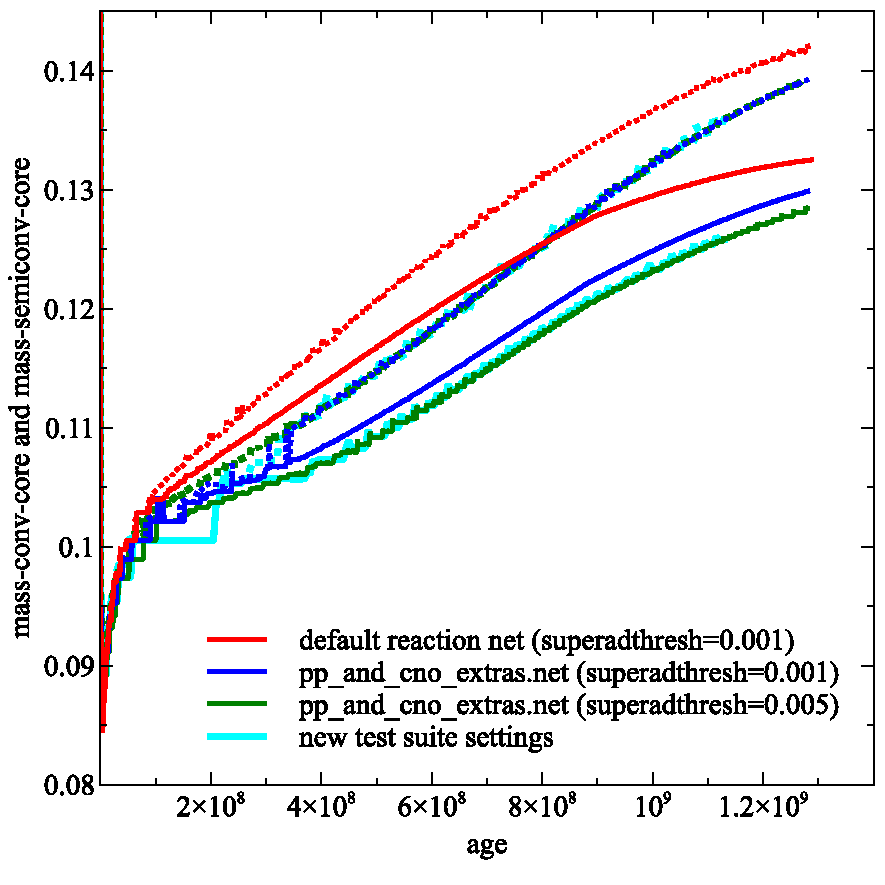
\includegraphics[width = 3.8in]{reactionnet.pdf}
	    \caption{}
	    \label{fig:2}
 \end{figure}

 \pagebreak












      


\end{document}
